\chapter{Test Access Port (TAP)}
\label{chap:TAP}

This chapter gives an overview about Test Access Port (TAP) and the interface signals that control the TAP controller. It contains the following sections 

\begin{itemize}
    \item \hyperref[sec:about-tap]{About TAP}
    \item \hyperref[sec:tap-controller]{TAP Controller}
\end{itemize}
\newpage

\section{About TAP}
\label{sec:about-tap}

TAP, uses the following signals to interface and support the operation of boundary scan.
\begin{itemize}
    \item \hyperref[subsec:tck]{Test Clock}
    \item \hyperref[subsec:tms]{Test Mode Select}
    \item \hyperref[subsec:tdi]{Test Data Input}
    \item \hyperref[subsec:tdo]{Test Data Output}
    \item \hyperref[subsec:trst]{Test Reset} (optional)
\end{itemize}

Table \ref{tab:top-port} shows the top level ports and description for the same.

\vspace{1cm}
\begin{table}[H]
    \caption{Top Level port description}
    \label{tab:top-port}
    \vspace{1cm}
    \begin{tabular}{l l l p{8cm}}

    \hline
         \textbf{Port} & \textbf{Name} & \textbf{Direction} & \textbf{Description}\\ \hline \hline
        \hyperref[subsec:tck]{TCK} & Test Clock & Input & The clock input to the BST circuitry.\\  \hline
        \hyperref[subsec:tms]{TMS} & Test Mode Select & Input & Provides the control signal to determine the transitions of the TAP controller state machine.\\ \hline
        \hyperref[subsec:tdi]{TDI} & Test Data Input & Input & Serial input pin for instructions as well as test data. Data is shifted in on the rising edge of TCK. \\ \hline
        \hyperref[subsec:tdo]{TDO} & Test Data Output & Output & Serial data output pin for instructions as well as test data. Data is shifted out on the falling edge of TCK. \\ \hline
        \hyperref[subsec:trst]{TRST} & Test Reset & Input & Asynchronous active low reset to reset the TAP controller, when TRST is applied to 0.
        \\ \hline
        \end{tabular}
\end{table}
\vspace{0.5cm}

\subsection{Test Clock, TCK}
\label{subsec:tck}
The dedicated TCK input is included so that the serial test data path between components can be used independently of component-specific system clocks, which may vary significantly in frequency from one component to the next. The provision of an independent clock helps ensure that test data can be moved to or from a component without changing the state of the on-chip system logic. 

The clock input to the BST circuitry. Some operations occur at the rising edge, while others occur at the falling edge. The clock input waveform should have a 50\% duty cycle.


\subsection{Test Mode Select, TMS}
\label{subsec:tms}
The value of the signal present at TMS at the time of a rising edge at TCK determines the next state of the TAP controller, the circuit that controls test operations. The signal presented at TMS shall be sampled by the test logic on the rising edge of TCK

\subsection{Test Data Input, TDI}
\label{subsec:tdi}
Serial test instructions and test data are received by the test logic at TDI. Values presented at TDI are clocked into the selected register (instruction or test data) on a rising edge of TCK.
The data pins (TDI and TDO) provide for serial movement of test data through the circuit. When data is being shifted from TDI toward TDO, test data received at TDI shall appear without inversion at TDO after a number of rising and falling edges of TCK determined by the length of the instruction or test data register selected.

\subsection{Test Data Output, TDO}
\label{subsec:tdo}
TDO is the serial output for test instructions and data from the test logic defined in this standard. Changes in the state of the signal driven through TDO shall occur only on the falling edge of TCK, i.e the contents of the selected register (instruction or data) are shifted out of TDO on the falling edge of TCK.

To help ensure a race-free operation, changes on TAP inputs (TMS and TDI) are clocked into the test logic defined by this standard on the rising edge of TCK while changes at the TAP output (TDO) occur on the falling edge of TCK. Similarly, for test logic able to drive or receive signals from system pins (e.g., the boundary-scan register), signals driven out of the component from the test logic change state on the falling edge of TCK, while those entering the test logic are clocked in on the rising edge. 

\subsection{Test Reset, TRST}
\label{subsec:trst}
The optional TRST input provides for asynchronous initialization, principally at power-up, of the TAP controller. TRST is required when the test logic does not power-up in a known and controlled state. If TRST is included in the TAP, the TAP controller shall be asynchronously reset to the Test-Logic-Reset state, when a logic 0 is applied to TRST. To avoid race conditions in the test logic, TMS should be held at 1 while the signal applied at TRST changes from 0 to 1.

\newpage

\section{TAP Controller}
\label{sec:tap-controller}

The IEEE Std. 1149.1 test access port (TAP) controller, a 16-state state machine clocked on the rising edge of TCK. 

TAP controller is a synchronous finite state machine that responds to changes at the TMS and TCK signals of the TAP, controls the behavior of the test logic, and maintains synchronization across all components on a test scan chain to permit shifting, capturing, and updating of data in the device.

\vspace{1cm}
\begin{figure}[H]
    \centering
    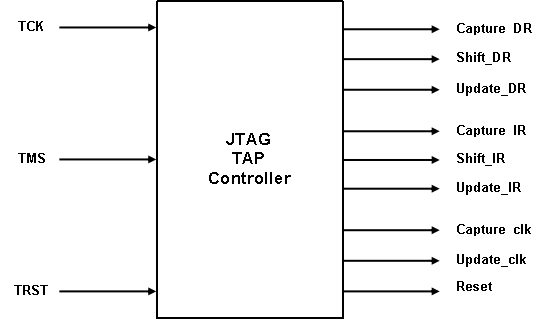
\includegraphics[width = 10cm]{images/jtag_tap_controller.png}
    \vspace{1cm}
    \caption{TAP Controller}
    \label{fig:tap-controller}
\end{figure}

\subsection{TAP Controller Ports}
\label{subsec:tap-controller-ports}

\begin{longtable}{l l p{9.5cm}}
    \caption{TAP controller port description}
    \label{tab:tap-ports}\\
    \hline
         \textbf{Port Name} & \textbf{Direction} & \textbf{Description}\\ \hline \hline
         \hyperref[subsec:tck]{TCK} & Input & Test Clock Input \\ \hline
         \hyperref[subsec:tms]{TMS} & Input & Test Mode Select Input \\ \hline
         \hyperref[subsec:trst]{TRST} & Input & Test Reset Input \\ \hline
         \hyperref[subsubsec:capture-dr]{Capture\_DR} & Output & This flag is set when the controller is in Capture\_DR State. It Controls the Capture operation in the Data Register Scan Path. \\ \hline
         \hyperref[subsubsec:shift-dr]{Shift\_DR} & Output & This flag is set when the controller is in Shift\_DR State. It controls the Shift operation in Data Register Scan Path. \\ \hline
         \hyperref[subsubsec:update-dr]{Update\_DR} & Output & This flag is set when the controller is in Update\_DR State. It controls the Update operation in the Data Register Scan Path. \\ \hline
         \hyperref[subsubsec:capture-ir]{Capture\_IR} & Output & This flag is set when the controller is in Capture\_IR State. It controls the Capture operation in the Instruction Register Scan Path. \\ \hline
         \hyperref[subsubsec:shift-ir]{Shift\_IR} & Output & This flag is set when the controller is in Shift\_IR State. It controls the Shift operation in the Instruction Register Scan Path. \\ \hline
         \hyperref[subsubsec:update-ir]{Update\_IR} & Output & This flag is set when the controller is in Update\_IR State. It controls the Update operation in the Instruction Register Scan Path. \\ \hline
         Capture\_clk & Output & It is the posedge of the TCK clock. This clock is used for Capture and Shift Operations. \\ \hline
         Update\_clk & Output & It is the negedge of the TCK clock. This clock is used for Update Operations. \\ \hline
         Reset & Output & This signal is set when the state is in \texttt{TEST\_LOGIC\_RESET} State.\\ \hline
\end{longtable}

\section{TAP Controller FSM}
\label{subsec:tap-fsm}

All state transitions of the TAP controller shall occur based on the value of TMS at the time of a rising edge of TCK. The transitions are as shown in Figure \ref{fig:tap-controller-fsm}.

\vspace{1cm}
\begin{figure}[H]
    \centering
    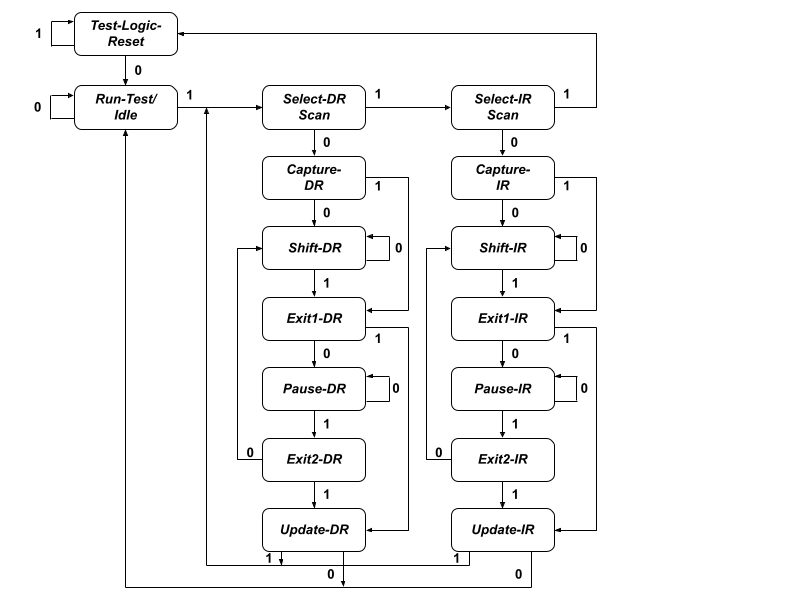
\includegraphics[width = 18cm]{images/tap_state_diagram.png}
    \vspace{1cm}
    \caption{TAP Controller FSM}
    \label{fig:tap-controller-fsm}
\end{figure}

\newpage

\subsection{TAP Controller Initialization}
\label{subsec:tap-controller-initial}

The TAP controller shall be forced into the Test-Logic-Reset controller state at power-up either by use of the TRST signal or as a result of circuitry built into the test logic or both.

The TAP controller shall not be initialized by operation of any system input, such as a system reset.

Where a dedicated reset pin (TRST) is provided to allow initialization of the TAP controller, initialization shall occur asynchronously (without dependence on TCK or any other clock) when the TRST input changes to the low logic level.

Where the TAP controller is initialized at power-up by operation of circuitry built into the test logic, the result shall be equivalent to that which would be achieved by application of a logic 0 to a TRST input.

\subsubsection{Test-Logic-Reset}
\label{subsubsec:test-logic-reset}
It resets the JTAG circuits. Whenever the TRST (optional) signal is asserted, it goes back to this state. The TAP controller state machine is designed so that, no matter what the initial state of the controller is, the Test-Logic-Reset state can be entered by holding TMS at high and pulsing TCK five times. Thus if we don’t have the TRST signal then we can still reset the circuit.

\subsubsection{Run-Test/Idle}
\label{subsubsec:run-test-idle}
In this state, the test logic in the IC is active only if certain instructions are present. For example, if an instruction activates the self test, then it is executed when the controller enters this state. The test logic in the IC is idle otherwise. The instruction does not change while the TAP controller is in this state.

\subsection{Select-IR Scan}
\label{subsec:select-ir}
This state controls whether or not to enter the Instruction Path. The Controller can return to the Test-Logic-Reset state otherwise. If TMS is held low and a rising edge is applied to TCK when the controller is in this state, then the controller moves into the Capture-IR state and a scan sequence for the instruction register is initiated. If TMS is held high and a rising edge is applied to TCK, the controller returns to the Test-Logic-Reset state.

\subsubsection{Capture-IR}
\label{subsubsec:capture-ir}
This is a temporary state in which a pattern of fixed logic values is parallel-loaded into specific bits of the instruction register shift-capture path on the rising edge of TCK. When the TAP controller is in this state and a rising edge is applied to TCK, the controller enters either the Exit1-IR state if TMS is held at 1 or the Shift-IR state if TMS is held at 0.

\subsubsection{Shift-IR}
\label{subsubsec:shift-ir}
In this state, the instruction register gets connected between TDI and TDO, and the captured pattern gets shifted on each rising edge of TCK from TDI to TDO. The instruction available on the TDI pin is also shifted into the instruction register. When the TAP controller is in this state and a rising edge is applied to TCK, the controller either enters the Exit1-IR state if TMS is held at 1 or remains in the Shift-IR state if TMS is held at 0.

\subsubsection{Exit1-IR}
\label{subsubsec:exit1-ir}
This state controls whether to enter the Pause-IR state if TMS holds low or Update-IR state if TMS holds high at the rising edge of TCK.

\subsubsection{Pause-IR}
\label{subsubsec:pause-ir}
This state allows shifting of the instruction register to be halted temporarily. The controller remains in this state while TMS is low. When TMS is set and a rising edge is applied to TCK, the controller moves on to the Exit2-IR state.

\subsubsection{Exit2-IR}
\label{subsubsec:exit2-ir}
If TMS is held high and a rising edge is applied to TCK while in this state, termination of the scanning process results, and the TAP controller enters the Update-IR controller state. If TMS is held low and a rising edge is applied to TCK, the controller enters the Shift-IR state.

\subsubsection{Update-IR}
\label{subsubsec:update-ir}
In this state, the bits in the instruction register shift-capture path are latched onto the parallel output on the falling edge of TCK. Once the new value has been latched, it becomes the current instruction. When the TAP controller is in this state and a rising edge is applied to TCK, the controller enters the Select-DR Scan state if TMS is held at 1 or the Run-Test/Idle state if TMS is held at 0.

\subsection{Select-DR Scan}
\label{subsec:select-dr}
This state controls whether to enter the Data Path or the Select-IR-Scan state. If TMS is held low and a rising edge is applied to TCK when the controller is in this state, the controller moves into the Capture-DR state and a scan sequence for the selected test data register is initiated. If TMS is held high and a rising edge is applied to TCK, the controller moves on to the Select-IR-Scan state.

\subsubsection{Capture-DR}
\label{subsubsec:capture-dr}
In this state, the data is parallel-loaded into the data registers selected by the current instruction on the rising edge of TCK. When the TAP controller is in this state and a rising edge is applied to TCK, the controller enters either the Exit1- DR state if TMS is held at 1 or the Shift-DR state if TMS is held at 0.

\subsubsection{Shift-DR}
\label{subsubsec:shift-dr}
This state is analogous to \hyperref[subsubsec:shift-ir]{Shift-IR} in the Instruction Path.

\subsubsection{Exit1-DR}
\label{subsubsec:exit1-dr}
This state is analogous to \hyperref[subsubsec:exit1-ir]{Exit1-IR} in the Instruction Path.

\subsubsection{Pause-DR}
\label{subsubsec:pause-dr}
This state is analogous to \hyperref[subsubsec:pause-ir]{Pause-IR} in the Instruction Path.

\subsubsection{Exit2-DR}
\label{subsubsec:exit2-dr}
This state is analogous to \hyperref[subsubsec:exit2-ir]{Exit2-IR} in the Instruction Path.

\subsubsection{Update-DR}
\label{subsubsec:update-dr}
This state is analogous to \hyperref[subsubsec:update-ir]{Update-IR} in the Instruction Path.